\documentclass[12pt]{article}
\usepackage[utf8]{inputenc}
\usepackage{amsfonts}
\usepackage{amsmath}
\usepackage{float}
\usepackage{siunitx}
\usepackage{amssymb}
\usepackage{enumitem}
\usepackage{mathtools}
\usepackage[brazil]{babel}
\usepackage{geometry}
\usepackage{graphicx}
\usepackage{bussproofs}
\usepackage[table]{xcolor}
\usepackage{gensymb}
\usepackage{hyperref}
\graphicspath{{.}}
\geometry{verbose,a4paper,left=2cm,top=2cm,right=3cm,bottom=3cm}
\title{Relatório EP2 - Laboratório de Métodos Numéricos}
\author{Lourenço Henrique Bogo - 11208005 \\ \& \\Miguel de Mello Carpi - 11208502}
\date{}
\linespread{1.5}
\newcommand{\real}{\mathbb{R}}
\newcommand{\product}[3]{\displaystyle\prod_{#1}^#2 #3}
\newcommand{\gsum}[3]{\displaystyle\sum_{#1}^#2 #3}
\newcommand{\mytitle}[1]{\textbf{\underline{#1}}}
\newcommand{\ring}[1]{\langle #1 \rangle}
\newcommand{\code}[1]{\mbox{\texttt{#1}}}

\begin{document}

\maketitle

\section{Decisões de Projeto}

\begin{description}
  
\item[\texttt{decompress.m}] Para ambos os métodos (bilienar e bicúbico), resolvemos os sistemas lineares colocando os dados na forma matricial e usando as funções de álgebra linear do \texttt{octave}. Utilizamos matrizes separadas para cada cor, pois achamos que o código ficaria mais claro.
  
\item[\texttt{compress.m}] Nessa função seguimos rigorosamente a especificação. Para fazer a retirada dos pixeis da imagem original, guardamos em um vetor os índices das linhas e colunas que queríamos remover da figura, e depois as substituímos por linhas e colunas vazias. Guardamos o resultado desse processo em uma imagem separada, para que possamos comparar, posteriormente, o produto final e a imagem original.
  
\item[\texttt{calculateError.m}] Aqui, também seguimos rigorasemente a especificação do EP, usando a função \texttt{norm} do \texttt{octave} para facilitar os cálculos.

  \mytitle{OBS:} Durante os testes percebemos que a função \texttt{norm} não estava funcionando em algumas versões do octave.
  As especificações que usamos para conseguir o resultado esperado foram:

  Distributor ID:  Ubuntu\\
  Description:  Ubuntu 20.04 LTS\\
  Release:  20.04\\
  Codename:  focal\\

  GNU Octave, version 5.2.0\\
  Octave was configured for "x86\_64-pc-linux-gnu"\\
  
\end{description}

\section{Testes}

\subsection{Imagens em preto e branco}
Para imagens em preto e branco, concluímos  que o algoritmo funciona bem, porém a parte visual tem uma aparência um pouco pior do que o esperado, já que o constraste entre as cores (preto e branco) é muito grande, realçando os erros.

Exemplos:
\begin{figure}[H]
  \centering
  \begin{minipage}{.5\textwidth}
    \centering
    
\includegraphics[width=.4\linewidth]{imagens/img_mickey/mickey.png}
    \caption{Original}
  \end{minipage}
  \begin{minipage}{.5\linewidth}
  \end{minipage}
  \begin{minipage}{.5\textwidth}
    \centering
    
\includegraphics[width=.4\linewidth]{imagens/img_mickey/mickey_1_7_1.png}
    \caption{Interpolado Bilinear k=7}
  \end{minipage}%
  \begin{minipage}{.5\textwidth}
    \centering
    
\includegraphics[width=.4\linewidth]{imagens/img_mickey/mickey_2_7_1.png}
    \caption{Interpolado Bicúbica k=7}
  \end{minipage}
\end{figure}

\begin{figure}[H]
  \centering
  \begin{minipage}{.5\textwidth}
    \centering
    
\includegraphics[width=.4\linewidth]{imagens/img_fogo/fogo.png}
    \caption{Original}
  \end{minipage}
  \begin{minipage}{.5\linewidth}
  \end{minipage}
  \begin{minipage}{.5\textwidth}
    \centering
    
\includegraphics[width=.4\linewidth]{imagens/img_fogo/fogo_1_6_1.png}
    \caption{Interpolado Bilinear k=6}
  \end{minipage}%
  \begin{minipage}{.5\textwidth}
    \centering
    
\includegraphics[width=.4\linewidth]{imagens/img_fogo/fogo_2_6_1.png}
    \caption{Interpolado Bicúbica k=6}
  \end{minipage}
\end{figure}

\subsection{Imagens coloridas}
Para imagens coloridas, o erro aproxima-se daquele que foi encontrado nas imagens em preto e branco. Porém, visualmente, estas imagens ficam melhores, uma vez que o degradê das cores disfarça as distorções.

Exemplos:
\begin{figure}[H]
  \centering
  \begin{minipage}{.5\textwidth}
    \centering
    
\includegraphics[width=.4\linewidth]{imagens/img_cmaismais/cmaismais.png}
    \caption{Original}
  \end{minipage}
  \begin{minipage}{.5\linewidth}
  \end{minipage}
  \begin{minipage}{.5\textwidth}
    \centering
    
\includegraphics[width=.4\linewidth]{imagens/img_cmaismais/cmaismais_1_7_1.png}
    \caption{Interpolado Bilinear k=7}
  \end{minipage}%
  \begin{minipage}{.5\textwidth}
    \centering
    
\includegraphics[width=.4\linewidth]{imagens/img_cmaismais/cmaismais_2_7_1.png}
    \caption{Interpolado Bicúbica k=7}
  \end{minipage}
\end{figure}

\begin{figure}[H]
  \centering
  \begin{minipage}{.5\textwidth}
    \centering
    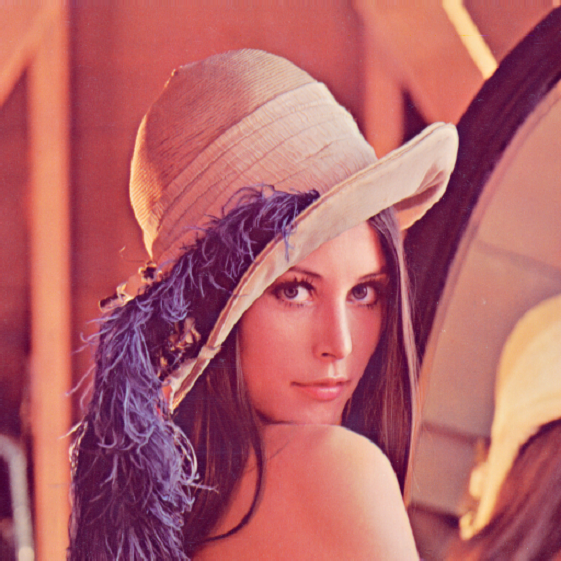
\includegraphics[width=.4\linewidth]{imagens/img_lenna/lenna.png}
    \caption{Original}
  \end{minipage}
  \begin{minipage}{.5\linewidth}
  \end{minipage}
  \begin{minipage}{.5\textwidth}
    \centering
    
\includegraphics[width=.4\linewidth]{imagens/img_lenna/lenna_1_7_1.png}
    \caption{Interpolado Bilinear k=7}
  \end{minipage}%
  \begin{minipage}{.5\textwidth}
    \centering
    
\includegraphics[width=.4\linewidth]{imagens/img_lenna/lenna_2_7_1.png}
    \caption{Interpolado Bicúbica k=7}
  \end{minipage}
\end{figure}

\newpage
\subsection{Funções $C^2$}
Para as imagens feitas a partir de funções $R^2\to R^3$ de classe $C^2$, os erros são \mytitle{muito} menores ($10^{-3}$ vezes menores, em média) do que os das imagens reais, sendo aqui que se acentua a diferença entre o método bilinear e o bicúbico.

O segundo método tem erro consistentemente menor que o primeiro para esse tipo de imagem. Aqui, também, recuperamos a imagem quase pefeitamente mesmo com enormes taxas de compressão.

Exemplos:
\begin{figure}[H]
  \centering
  \begin{minipage}{.5\textwidth}
    \centering
    
\includegraphics[width=.4\linewidth]{imagens/img_f/f1.png}
    \caption{Original}
  \end{minipage}
  \begin{minipage}{.5\linewidth}
  \end{minipage}
  \begin{minipage}{.5\textwidth}
    \centering
    
\includegraphics[width=.4\linewidth]{imagens/img_f/f1_1_7_1.png}
    \caption{Interpolado Bilinear k=7}
  \end{minipage}%
  \begin{minipage}{.5\textwidth}
    \centering
    
\includegraphics[width=.4\linewidth]{imagens/img_f/f1_2_7_1.png}
    \caption{Interpolado Bicúbica k=7}
  \end{minipage}
\end{figure}

\begin{figure}[H]
  \centering
  \begin{minipage}{.5\textwidth}
    \centering
    
\includegraphics[width=.4\linewidth]{imagens/img_f/f3.png}
    \caption{Original}
  \end{minipage}
  \begin{minipage}{.5\linewidth}
  \end{minipage}
  \begin{minipage}{.5\textwidth}
    \centering
    
\includegraphics[width=.4\linewidth]{imagens/img_f/f3_1_7_1.png}
    \caption{Interpolado Bilinear k=7}
  \end{minipage}%
  \begin{minipage}{.5\textwidth}
    \centering
    
\includegraphics[width=.4\linewidth]{imagens/img_f/f3_2_7_1.png}
    \caption{Interpolado Bicúbica k=7}
  \end{minipage}
\end{figure}

\subsection{Funções não $C^2$}
Para as imagens reais e as que não são feitas com funções de classe $C^2$, observamos que a bicúbica não é necessariamente melhor que a bilinear. Isso porque, na interpolação bicúbica, as derivadas de primeira e segunda ordem e suas continuidades são necessárias para o método funcionar bem, enquanto no bilinear não são tão importantes.

\begin{figure}[H]
  \centering
  \begin{minipage}{.5\textwidth}
    \centering
    
\includegraphics[width=.4\linewidth]{imagens/img_f/f4.png}
    \caption{Original}
  \end{minipage}
  \begin{minipage}{.5\linewidth}
  \end{minipage}
  \begin{minipage}{.5\textwidth}
    \centering
    
\includegraphics[width=.4\linewidth]{imagens/img_f/f4_1_7_1.png}
    \caption{Interpolado Bilinear k=7}
  \end{minipage}%
  \begin{minipage}{.5\textwidth}
    \centering
    
\includegraphics[width=.4\linewidth]{imagens/img_f/f4_2_7_1.png}
    \caption{Interpolado Bicúbica k=7}
  \end{minipage}
\end{figure}

\newpage
\section{Como o h influencia a interpolação?}
Após repetidos testes com diferentes valores de h, concluímos que não há alterações nas interporlações.

\mytitle{OBS} Se o h for 0, ocorrerá divisão por 0 e o programa não funcionará; se o h for um número muito pequeno, ocorrerá cancelamento catastrófico.

\section{Erro}
O erro já foi discutido nas outras seções, mas aqui resumiremos o seu comportamento:

\begin{itemize}
  
\item Para funções de classe $C^2$, o erro é muito menor na bicúbica (da ordem de $10^{-6}$) do que na bilinear (da ordem de $10^{-5}$).
  
\item Para as imagens reais, o erro parece não ter muita conexão com o método utilizado, podendo ser maior ou menor em qualquer dos casos. Aqui, os erros são, em média, da ordem de $10^{-2}$.
  
\end{itemize}

Para os testes feitos nesse secção foi usado k = 7.

Erros obtidos com os exemplos:
\begin{center}
  \begin{tabular}{||c | c | c | c | c||} 
    \hline
    Imagem & Bilin k=7 & Bicub k=7 & Bilin k=3 & Bicub k=3 \\ [0.5ex] 
    \hline\hline
    $f(x, y) = (\sin{x}, \frac{\sin{x}+\sin{y}}{2}, \sin{x})$ & 23165e-5 & 94246e-6 & 79225e-6 & 80150e-6 \\ 
    \hline
    Lenna & 29432e-2 & 29960e-2 & 14894e-2 & 14537e-2 \\
    \hline
    C++ & 33827e-2 & 34192e-2 & 13854e-2 & 13265e-2 \\
    \hline
    Mickey & 62983e-2 & 65166e-2 & 29824e-2 & 27828e-2 \\ [1ex]
    \hline
  \end{tabular}
\end{center}

\mytitle{OBS:} No caso k=3, a bilinear foi melhor que a bicúbica para a função de $\real^2\to \real^3$. Uma vez que a taxa de compressão era muito pequena, os erros de aproximação da bicúbica foram mais significativos que o próprio polinômio em si. Para efeito de comparação, segue uma tabela com taxas de compressão maiores para a mesma função, mostrando que a bicúbica é melhor:

\begin{center}
  \begin{tabular}{||c | c | c  | c | c||} 
    \hline
    Imagem & Bilin k=139 & Bicub k=139 & Bilin k=279 & Bicub k=279\\[0.5ex] 
    \hline\hline
    $f(x, y) = (\sin{x}, \frac{\sin{x}+\sin{y}}{2}, \sin{x})$ & 70202e-3 & 28071e-3 & 27732e-2 & 16950e-2 \\[1ex]
    \hline
  \end{tabular}
\end{center}

Notamos, também, que o erro foi da ordem de $10^{-2}$ mesmo com uma taxa de compressão gigantesca ($139$).

\newpage
\section{Múltiplas Compressões}
Ao comparar os erros da compressão direta e das múltiplas compressões (tabela a seguir) percebemos que, ao descomprimir três vezes com k=1 e descomprimir uma vez com k=7, o resultado foi exatamente o mesmo (as diferenças vistas nos bicúbicos foram causadas por erro de aproximação).

\begin{center}
  \begin{tabular}{||c | c | c  | c | c||} 
    \hline
    Imagem & Bilin k=7 & Bicub k=7 & Bilin 3 (k=1) & Bicub 3 (k=1)\\[0.5ex] 
    \hline\hline
    $f(x, y) = P(x, y)$ & 18058e-3 & 12069e-3 & 18059e-3 & 11935e-3 \\
    \hline
    Lenna & 29432e-2 & 29960e-2 & 29432e-2 & 29894e-2 \\[1ex]
    \hline    
  \end{tabular}
\end{center}

\mytitle{PS:}$P(x, y) = x^5 + (x - y^2)^2 - x^3, x^2 + x^4 + x^6 - y^5 - y^3 - y, (x^3 - y^3)^2$.
\\

Mas por que isso?

Cada vez que descomprimimos uma imagem de $p$ pixeis com um certo $k$, o número de pontos da nova imagem será aproximadamente $(k+1)p$. Ou seja, ao descomprimir uma imagem com $k=7$, o novo número será em torno de $8p$. Ao descomprimir três vezes com $k=1$, o novo número será em torno de $(2(2(2p))) = 8p$, resultando em imagem e números de pixeis iguais, já que o algoritmo que achou os pixeis é o mesmo.

\end{document}